\subsection{Modalities}

\begin{figure}
    \centering
    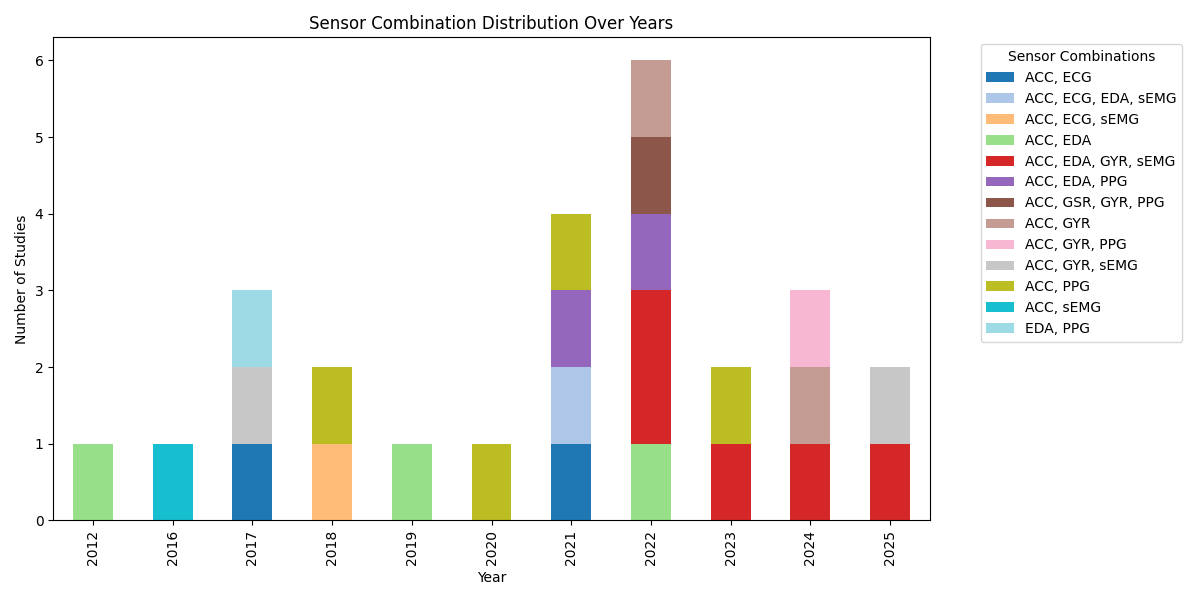
\includegraphics[width=1\textwidth]{Discussion/figures/Sensor_Combination_Distribution_Over_the_Years.png}
    \caption{Sensor combination distribution over the years.}
    \label{fig:sensor_comb_over_years}
\end{figure}

\subsubsection{Detection}
Across the 26 reviewed studies, non-EEG multimodal sensor setups show strong potential for motor seizure detection and management methods.

However, direct comparisons are difficult due to methodological and population differences. Nevertheless. The (ACC + GYR + EDA + sEMG) combination consistently performed well (table \ref{tab:modalities}) , likely because motion sensors (ACC, GYR, sEMG) ensure reliable detection, while EDA reduces false alarms. Notably, sEMG enabled rapid detection with a short delay of 11.7 s  \cite{De_Cooman2018-pq}, supporting its value for timely intervention.

The ACC + EDA combination is also among the best performers, offering fewer sensors, lower costs, and simpler data processing. This may be due to EDA’s sensitivity to sympathetic activation at seizure onset in both children and adults \cite{Casanovas_Ortega2022-yx}, and its lower susceptibility to motion artifacts compared to signals like PPG  \cite{Ismail2021-fs}. EDA increases have also been linked to postictal EEG suppression (PGES), a SUDEP risk factor \cite{Barot2019-nx,Regalia2019-ch}, underscoring its preventive potential. However, some studies reported poor EDA performance alone or with other sensors \cite{Yu2023-ss,Tang2021-td}, possibly due to age-related EDA variability noted in pediatric research \cite{Ge2023-ab}, emphasizing the need for age-adaptive algorithms.

Other physiological sensors such as PPG have also been widely used to extract biomarkers such as HR \cite{Cogan2017-lg,Nasseri2021-xn,Vakilna2024-hk,Xu2022-tx,Jiang2022-zu,Arends2018-ew}, HRV \cite{Vakilna2024-hk,Jiang2022-zu}, SpO2 \cite{Cogan2017-lg}, and BVP \cite{Yu2023-ss,Nasseri2021-xn,Tang2021-td}. Among these, BVP showed strong potential, consistently performing well across seizure types. This aligns with an observational study \cite{Mohammadpour_Touserkani2020-tk} showing that not only HR but also PPG features like smoothness and slope vary with seizure timing, enhancing BVP-based detection accuracy.

ECG has also been used to derive HR \cite{Hegarty-Craver2021-hk,De_Cooman2018-pq,Van_Andel2017-yx} and HRV \cite{Hegarty-Craver2021-hk}, with some studies reporting that unimodal ECG systems can achieve performance comparable to multimodal approaches \cite{Hegarty-Craver2021-hk,De_Cooman2018-pq}. However, ECG was used less frequently in the reviewed studies, largely due to its susceptibility to motion artifacts \cite{Van_Andel2017-yx}, impractical electrode placement, and high inter-patient variability \cite{Van_Andel2017-yx,De_Cooman2018-pq}.

Because of these limitations, ECG has mostly been used in nocturnal studies \cite{Van_Andel2017-yx,De_Cooman2018-pq}. This is relevant since SUDEP ofter occurs at night \cite{Friedman2022-mo}. HR and HRV remain potential SUDEP biomarkers \cite{Barot2019-nx}, suggesting ECG’s dual role in seizure detection and SUDEP monitoring SUDEP-related autonomic changes.

Some studies explored non-traditional biomarkers for seizure detection, with several showing performance comparable to or exceeding established biomarkers. Hamlin et al. \cite{Hamlin2021-sd} used audio features from a microphone, identifying them among the top ten discriminative features establishing separability between seizure and non-seizure data in five patients. Wang et al. \cite{Wang2025-ql} found that adding or replacing ACC/GYR with attitude angles (pitch or roll) improved performance across all models due to their better resistance to non-seizure motion interference. Xu et al. \cite{Xu2022-tx} used number of wrist movements (NOWM) instead of raw ACC data to better distinguish seizures from normal movements.

Beyond sensor type, placement and signal quality significantly affect detection performance. Tang et al. \cite{Tang2021-td} found inconsistent signals from different body sites. Arends et al. \cite{Arends2018-ew} excluded participants with abnormal movements or darker skin due to poor PPG signal quality which was affected by light intensity. The chest-worn sensor in Hegarty-Craver et al. \cite{Hegarty-Craver2021-hk} missed limb movements, reducing the device's overall sensitivity, while Cogan et al. \cite{Cogan2017-lg} reported data loss from SpO2 sensors.

Future studies should validate these biomarkers while optimizing sensor placement, as outcomes vary by location  \cite{Milosevic2016-ee,De_Cooman2018-pq}. They should also diversify cohorts and develop personalized models to address physiological variability, particularly for patient-dependent signals like HR and HRV.

\subsubsection{Prediction and Forecasting}
Despite differing methods and objectives, the three prediction studies collectively support the feasibility of using Empatica E4 wristband data with machine or deep learning for seizure prediction. Vieluf et al. \cite{Vieluf2023-ta,Vieluf2023-zv} showed that autonomic signals (EDA and PPG-from which HR/HRV are derived) could successfully identify pre-ictal periods in many patients. Meisel et al. \cite{Meisel2020-ii}achieved the highest performance by using all E4 modalities (EDA, PPG/BVP, ACC, TEMP), confirming the superiority of multimodal sensor combinations observed in detection studies.

PPG-derived biomarkers appear to be key seizure predictors. While two studies \cite{Vieluf2023-ta,Vieluf2023-zv} identified HR as predictive, clinical observations \cite{Mohammadpour_Touserkani2020-tk} showed that raw PPG features—such as frequency, smoothness, and slope—change during peri- and post-ictal phases, suggesting added predictive value. Future research should evaluate raw PPG signals directly in larger, more diverse cohorts.